\documentclass{article}
\usepackage{graphicx}
\usepackage[margin=2.5cm]{geometry}
\usepackage[labelfont=bf]{caption}
\usepackage{color}
\usepackage{xcite}
\usepackage{amsmath}
%\usepackage{natbib}
\usepackage{subcaption}
\usepackage{multirow}

\renewcommand{\textfraction}{1.0}
\renewcommand{\floatpagefraction}{.9}
\newcommand\revised[1]{\textcolor{red}{#1}}
\renewcommand{\topfraction}{0.9}    % max fraction of floats at top
\renewcommand{\bottomfraction}{0.8} % max fraction of floats at bottom
\renewcommand{\textfraction}{0.07}  % allow minimal text w. figs

\makeatletter 
\renewcommand{\thefigure}{S\@arabic\c@figure} 
\renewcommand{\thetable}{S\@arabic\c@table} 

\newcommand{\figdeconv}{2}

\externalcitedocument{betternorm}

\usepackage{url}
\urlstyle{same}

\begin{document}

\begin{titlepage}
\vspace*{3cm}
\begin{center}

{\LARGE
Computing normalization factors for single-cell RNA-seq data: avoiding problems with zero counts
\par}

\vspace{0.75cm}

{\Large 
    \textsc{Supplementary Materials}
\par
}
\vspace{0.75cm}

\large
by

\vspace{0.75cm}
Aaron T. L. Lun$^{1}$ and Karsten Bach$^{2}$

\vspace{1cm}
\begin{minipage}{0.9\textwidth}
\begin{flushleft} 
$^1$Cancer Research UK Cambridge Institute, University of Cambridge, Li Ka Shing Centre, Robinson Way, Cambridge CB2 0RE, United Kingdom \\[6pt]
$^2$European Bioinformatics Institute (EMBL-EBI), Wellcome Genome Campus, Hinxton, Cambridge CB10 1SD, United Kingdom \\[6pt]
\end{flushleft}
\end{minipage}

\vspace{1.5cm}
{\large \today{}}

\vspace*{\fill}
\end{center}
\end{titlepage}

\section{Implementation details for the deconvolution method}

\subsection{Summation and deconvolution with linear equations}
Define the adjusted expression of gene $i$ as $\pi_{ij} = y_{ij}T_j^{-1}$, where $T_j$ is a constant adjustment factor for cell $j$ (usually the library size).
This means that $E(\pi_{ij}) =\theta_j\lambda_{is} T_j^{-1}$.
Further assume that we have an arbitrary set of cells $\mathcal{S}_k$.
Denote the sum of $\pi_{ij}$ across $\mathcal{S}_k$ as $s_{ik}$ for gene $i$.
The values of $s_{ik}$ across all genes constitute an overall expression profile for the pool of cells corresponding to $\mathcal{S}_k$.
The expectation of $s_{ik}$ is equal to 
\[
    E(s_{ik}) = \lambda_{is} \sum_{j \in \mathcal{S}_k} \theta_j T_j^{-1}\;.
\]
Define $u_{i}$ as the mean of expression values for gene $i$ across all $N$ cells in the entire data set.
The values of $u_{i}$ across all genes represent the expression profile for an averaged reference pseudo-cell.
The cell pool for set $\mathcal{S}_k$ is then normalized against this reference pseudo-cell.
Let $r_{ik}$ denote the ratio of $s_{ik}$ to $u_{i}$ for a non-DE gene $i$.
The expectation of $r_{ik}$ represents the size factor for the pooled cells in $\mathcal{S}_k$, and is written as
\begin{equation}
    E(r_{ik}) \approx \frac{E(s_{ik})}{E(u_{i})} 
    = \frac{\sum_{\mathcal{S}_k} \theta_j T_j^{-1}}{ N^{-1} \sum_{\mathcal{S}_0} \theta_j T_j^{-1}} 
    = \frac{\sum_{\mathcal{S}_k} \theta_j T_j^{-1}}{C}
    \label{eqn:linear_single}
\end{equation}
where $C$ is a constant that does not depend on the gene, cell or $\mathcal{S}_k$.
The approximation assumes that $u_{i}$ is stably estimated 
    -- this is not unreasonable for data sets with hundreds of cells, where variability relative to the mean should decrease due to the law of large numbers.
$E(r_{ik})$ is estimated by taking a robust average (i.e., the median) of $r_{ik}$ across $i$.
Robustness protects the average against DE genes with extreme ratios.

The estimated value of $E(r_{ik})$ for the set can be used to obtain estimates for $\theta_j$ for each cell.
A linear equation is set up based on the expression in Equation~\ref{eqn:linear_single}, 
by replacing $E(r_{ik})$ with its estimate and treating the $\theta_j T_j^{-1}$ as unknown parameters to be estimated.
The constant $C$ can be set to unity and ignored, as it does not contribute to the relative differences between size factors.
Repeating the estimation of $E(r_{ik})$ for different sets of cells in $\mathcal{S}_{ik}$ will generate an overdetermined system of linear equations, 
    in which the $\theta_j T_j^{-1}$ for each $j$ is represented at least once.
This system can be solved with standard least-squares methods to obtain estimates of $\theta_j T_j^{-1}$ for all cells 
    (this represents ``deconvolution'' of the cell pool factors to the factors for the individual cells, hence the name).
Multiplication by $T_j$ for each cell will yield an estimate of $\theta_j$.

This approach may seem somewhat circuitous, given that $\theta_j$ could be estimated directly from the counts for each individual cell.
However, summation reduces the number of stochastic zeroes that cause problems in existing methods.
As a result, ratios computed from pooled expression profiles are more accurate.
This improvement will propagate back to the $\theta_j$ estimates for each $j$ when the linear system is solved.

\subsection{Obtaining sensible least-squares solutions}
The linear system can be solved using standard methods, such as those based on the QR decomposition.
However, with such methods, it is theoretically possible to obtain negative estimates for $\theta_j$.
Such values are obviously nonsensical as counts cannot be scaled to negative values.
One situation in which this might occur involves data with a large spread of $\theta_jT_j^{-1}$ values, 
    such that the true value of $\theta_jT_j^{-1}$ is already close to zero for some cells.
Errors in estimation may then be sufficient to push the estimated $\theta_j$ below zero.
Protection is provided by using linear inverse models in the limSolve package (v1.5.5.1, \url{https://cran.r-project.org/web/packages/limSolve/index.html}) to constrain the estimates to non-negative values.
This will not provide sensible size factor estimates for the offending cells -- these are set to zero and should be removed --
    but will ensure that the estimates for other cells are not distorted by negative values elsewhere in the system.

The value of $T_j$ is typically set to the observed library size for each cell.
This ensures that the sum $s_{ik}$ is not dominated by a small number of very large libraries.
Information from each cell will be weighted equally when computing the median ratio for each set, regardless of library size.
It also reduces the risk of obtaining negative estimates for small libraries.
Such libraries have small $\theta_j$ and would be unduly influenced by (relatively) large estimation errors for cells with larger libraries.
The fact that the observed library size is variable is largely irrelevant, as the deconvolution procedure is valid for arbitrary positive values of $T_j$.

\subsection{Clustering to weaken the non-DE assumption}

\subsubsection{Overview}
This approach makes some moderately strong assumptions regarding the nature of DE across the data set.
The use of the median is only valid when less than 50\% of genes are DE in any direction in the cell pool compared to the reference pseudo-cell,
    i.e., less than 50\% of genes can be upregulated and less than 50\% of genes can be downregulated.
If more DE genes are present, the median will not represent a robust average across non-DE genes.
This condition generally requires a proportion of genes to be constantly expressed across all cells in the data set 
    -- otherwise, all genes would be DE against the average in at least one pool of cells -- 
    and is only guaranteed to be true when that proportion is equal to or greater than 50\% of all genes.
This is similar to that required for DESeq normalization where an average reference is also used.

\subsubsection{Deconvolution on clustered cells}
To reduce the strength of the non-DE assumption, cells can be clustered based on their expression profiles.
The deconvolution method is then applied to the cells in each cluster $\mathcal{C}$ separately,
    where the sets $\mathcal{S}_k$ are nested within each $\mathcal{C}$.
This normalizes each cell pool of $\mathcal{S}_k$ to a cluster-specific reference pseudo-cell for $\mathcal{C}$,
    yielding a cluster-specific size factor of $f_{j}'$ for cell $j \in \mathcal{C}$ after deconvolution.
These cluster-specific size factors must be rescaled before they can be compared between clusters.
To do so, the reference pseudo-cells for all clusters are normalized against each other.
This is done by selecting a single ``baseline'' pseudo-cell against which all other pseudo-cells are normalized.
The median ratio $\tau_{\mathcal{C}}$ of the expression values is computed for the pseudo-cell of each cluster against the baseline pseudo-cell
    (obviously, the cluster chosen as the baseline will have $\tau_{\mathcal{C}}=1$).
The overall size factor for cell $j$ in cluster $\mathcal{C}$ is subsequently defined as $f_j = f_{j}'\tau_{\mathcal{C}}$.

% This is justified by considering normalization factors; you multiply the normalization factor within clusters with that between clusters to get the overall factor 
% (independent of library size), then you multiply by the library size to get the size factors. 
% The same applies here, except that you multiply by library size first to get the within-cluster size factors, then you multiply between clusters.
% Or, in other words, the within-cluster size factors capture library size differences and additional within-cluster differences;
% you only need to multiply by additional between-cluster differences to get the overall size factors 
% (i.e., you don't need to compute the size factors between clusters, only the normalization factors).

The use of within-cluster normalization reduces the amount of DE between cells, as all cells in each cluster have similar expression profiles.
This avoids inaccurate estimation of the size factors due to violations of the non-DE assumption.
Moreover, the pseudo-cells are normalized in pairwise comparisons to a baseline.
This weakens the assumption as a non-DE majority is only required across pairs of pseudo-cells/clusters, rather than across the entire data set.
For example, in the simulation with varying magnitude of DE, only 60\% of genes are DE between any two subpopulations, while 90\% of genes are DE across all subpopulations.

In general, cluster-specific normalization requires some caution.
Done incorrectly, this may introduce artificial differences between cells in different clusters, 
    such that the statistical rigour of downstream analyses (e.g., to detect DE between clusters) would be compromised.
However, such problems are avoided here by using a two-step normalization strategy.
The first normalization step removes any systematic differences between cells in each cluster, 
    while the second normalization between pseudo-cells removes any differences between clusters.
The end result is that differences between all cells in all clusters are removed.
This is equivalent to the outcome of a hypothetical one-step method that does not use cluster information (and is robust to DE and stochastic zeroes, unlike existing methods).
Moreover, normalization accuracy in Figure~\figdeconv{} is unaffected by the use of clustering prior to deconvolution, which suggests that this approach is valid.

\subsubsection{Implementation details of the clustering approach}
Any clustering technique can be used to group cells with similar expression profiles.
We favour a correlation-based approach using $1-\rho_{xy}$ as the distance, where $\rho_{xy}$ denotes Spearman's rank correlation coefficient between the counts of cells $x$ and $y$.
In this manner, a distance matrix is constructed between all pairs of cells.
Hierarchical clustering is then performed on this matrix using Ward's clustering criterion.
A dynamic tree cut is used to define clusters of cells using the dynamicTreeCut package v1.62 (\url{https://cran.r-project.org/web/packages/dynamicTreeCut/index.html}).
This is done so that each cluster contains a minimum number of cells (200 by default) required for stable deconvolution.
Correlation-based methods are attractive as they are insensitive to global scaling of the expression values in each cell.
Prior normalization is not required, which avoids a circular dependence between normalization and clustering.
Alternatively, one can use known aspects of the data set as clusters, e.g., treatment conditions, batches.
If such information is available, empirical clustering may not be required.
This reduces computational work and avoids potential errors.

By default, the baseline pseudo-cell is chosen from the cluster where the mean library size per cell is equal to the median of the mean library size across all clusters
    (or, for an even number of clusters, the cluster with the smallest mean library size above the median).
This uses the mean library size as a rough proxy for cell similarity.
The baseline cluster is likely to be least dissimilar to every other cluster, which reduces the amount of DE during pairwise normalization between pseudo-cells.
More intelligent choices of the baseline can be used if the similarities between clusters are known, e.g., from visualization after dimensionality reduction.

Systematic zeroes within each cluster are also removed prior to deconvolution in that cluster.
This removes genes that have only zero counts across all cells in the cluster.
Such genes provide no information for normalizing between cells in the same cluster, and their removal will not affect the cluster-specific size factor estimates.
However, these genes are retained during rescaling of the size factors between clusters.
This is because they will have non-zero counts in at least one cluster (assuming that systematic zeroes across the entire data set have already been removed).
Removal of such genes will distort the median ratio between pseudo-cells and lead to biased size factor estimates, as described previously for the existing methods.

\subsection{Selecting cell pools to sum}
The pool of cells in each $\mathcal{S}_{ik}$ is chosen to consist of similar library sizes.
Cells in a given cluster are ordered by their total counts and partitioned into two groups, depending on whether the ranking of each cell is odd or even.
These cells are arranged in a ring, with odd cells on the left and even cells on the right.
Conceptually, one can start at the 12 o'clock position on the ring, for the largest libraries; moving clockwise through the even cells with decreasing library size;
reaching the smallest libraries at 6 o'clock; and then, continuing to move clockwise through the odd cells with increasing library size (Figure~\ref{fig:library_ring}).
For summation, a sliding window is moved cell-by-cell across this ring where each window contains the same number of cells.
These cells are used to define a single instance of $\mathcal{S}_{k}$.
Thus, each window defines a separate equation in the linear system.
The use of a ring means that the window is still defined at the smallest and largest libraries.
In contrast, sliding a window across a linear ordering of cells will result in truncated windows at the boundaries.

\begin{figure}[bt]
    \begin{center}
        \includegraphics[width=0.5\textwidth]{pics/library_ring.pdf}
    \end{center}
    \caption{
        Ring arrangement of cells ordered by library size.
        Each circle represents a cell where the size of the circle corresponds to the library size of that cell.
        Even- and odd-ranking cells lie on opposite sides, with the largest and smallest libraries at the top and bottom, respectively.
        Cells lying in a window of length 4 are highlighted in red.
        Different instances of the window are obtained by sliding the window across the ring.
    }
    \label{fig:library_ring}
\end{figure}

The pooling of cells with similar library sizes is designed to provide some robustness to DE.
Specifically, the library size is used as a rough proxy for cell similarity.
This is motivated by the fact that different cell types tend to have systematic differences in the library sizes, 
    e.g., due to type-specific differences in total RNA or capture efficiency.
Summation of cells with similar library sizes (and by implication, similar expression profiles) reduces the number of DE genes in the cell pool relative to the pseudo-cell.
This further weakens the non-DE assumption that is required by the deconvolution approach.
Note that this pooling strategy is performed on cells within a single cluster at a time.
It complements the use of clustering by protecting against any residual DE within each cluster.
This is especially true for heterogeneous populations that are difficult to partition, or in cases where larger clusters must be formed due to low numbers of cells.

% In small samples, it mightn't matter whether or not the cells have similar expression profiles;
% DE anywhere in the data set will contaminate the average reference anyway, so the amount of DE in each cell pool relative to the pseudo-cell would be the same.
% However, if the cluster is large enough, minor DE will average out in the pseudo-cell.
% Then we definitely can see an advantage from summing similar cells at a time in each cell pool. 

The total number of equations in the linear system is equal to the number of cells.
The $\theta_jT_j^{-1}$ term for each cell is represented in $w$ equations, where $w$ denotes the size of the window.
By using different values of $w$, additional equations can be added to improve the precision of the estimates. 
Specifically, values of $w$ are set to 20, 40, 60, 80 and 100.
These are large enough to obtain stable sums yet small enough to maintain resolution, i.e., by ensuring that cells with very different library sizes are not summed together.
This increases the total number of equations in the system and means that each $\theta_j$ is represented in 300 equations. 

An additional set of equations is added to ensure that the system is solvable.
In each equation, the $\theta_jT_j^{-1}$ for each cell is equated to the size factor estimated directly from its single-cell counts.
These equations are assigned very low weights compared to those of the other equations involving summed cells, equal to $10^{-6}$ and unity respectively.
A weighted least-squares approach is then applied to solve the linear system.
In the matrix containing the coefficients of the linear system, the incorporation of the additional equations ensures that the columns are linearly independent.
This ensures that a single solution can be obtained.
Due to their low weights, the additional equations will not contribute substantially to the weighted least-squares solution.
This means that the estimated values will be driven primarily by the equations for the summed cells.

\section{Deconvolution is inconsistent with spike-in normalization}
The brain data set also contains counts for ERCC spike-in genes that are commonly used for normalizing scRNA-seq data.
Briefly, a constant quantity of spike-in RNA is added to each cell and processed with the cellular RNA \cite{stegle2015computational}.
Upon sequencing and quantification, differences in the coverage of spike-in genes between cells are interpreted as cell-specific biases and removed.
At its simplest, spike-in normalization uses the total count across the spike-in genes as the size factor for each cell.
This is similar to library size normalization with the counts for the cellular genes, but is more robust as no DE is expected across cells for a constant spike-in set.
Problems with stochastic zeroes are avoided, and the assumption of a non-DE majority is not required.
However, spike-in normalization does assume that the same quantity of spike-in RNA can be added to each cell \cite{robinson2010scaling,marinov2014singlecell}.
It also assumes that the spike-ins behave similarly to the cellular transcripts \cite{grun2015design}.
Violations of these assumptions may compromise performance, as observed in some bulk RNA-seq data sets \cite{risso2014normalization}.

Examination of the data indicates that no correlation -- qualitative or quantitative -- 
    exists between the sets of size factors from spike-in and the other normalization methods (Figure~\ref{fig:real_spike}).
This is attributable to the differences in the underlying assumptions of each method.
If most genes are DE, deconvolution and the existing methods will be incorrect and spike-in normalization will be more accurate.
Conversely, spike-in normalization will be incorrect if spike-ins are not added precisely or if spike-in and cellular transcripts behave differently during library preparation.
These results suggest that the validity of each assumption requires some consideration before normalization.
For example, the similarity of the input cell types can be used to gauge the appropriateness of the non-DE assumption. 
Here, over half of the cells are classified as neuronal \cite{zeisel2015brain}, so a non-DE majority of genes is not entirely unreasonable.
Obviously, the truth of each assumption is largely unknown, so it is difficult to definitively determine the correct method for any given data set.

\begin{figure}[btp]
\begin{center}
    \begin{minipage}{0.33\textwidth}
        \includegraphics[width=\textwidth,trim=0mm 5mm 0mm 15mm,clip]{realdata/Zeisel_ERCCvSF.pdf}
        \subcaption{}\label{subfig:spike_sf}
    \end{minipage}
    \begin{minipage}{0.33\textwidth}
        \includegraphics[width=\textwidth,trim=0mm 5mm 0mm 15mm,clip]{realdata/Zeisel_ERCCvTMM.pdf}
        \subcaption{}\label{subfig:spike_tmm}
    \end{minipage} \\ 
    \begin{minipage}{0.33\textwidth}
        \includegraphics[width=\textwidth,trim=0mm 5mm 0mm 15mm,clip]{realdata/Zeisel_ERCCvLib.pdf}
        \subcaption{}\label{subfig:spike_lib}
    \end{minipage} 
    \begin{minipage}{0.33\textwidth}
        \includegraphics[width=\textwidth,trim=0mm 5mm 0mm 15mm,clip]{realdata/Zeisel_ERCCvDeconv.pdf}
        \subcaption{}\label{subfig:spike_sum}
    \end{minipage}
\end{center}
    \caption{
        Comparisons between the estimated size factors from spike-in normalization to those from (\subref{subfig:spike_sf}) DESeq, (\subref{subfig:spike_tmm}) TMM,
            (\subref{subfig:spike_lib}) library size normalization or (\subref{subfig:spike_sum}) the deconvolution method for all cells in the brain data set.                  
        All sets of size factors were scaled to have a median of unity.
        Axes are shown on a log-scale.
    }
    \label{fig:real_spike}  
\end{figure}

Of greater biological relevance is the fact that spike-in normalization preserves differences in cell size and total RNA content.
In contrast, deconvolution and the existing methods will remove such differences.
This is because they affect all genes within each cell and are subsequently treated as part of the cell-specific bias.
Whether or not this is appropriate depends on whether cell size differences are of interest to the researcher.
In some scenarios, this may be the case such that spike-ins should be used, e.g., when studying cycling cells with differences in total RNA.
For other applications, cell size may be a confounding variable that needs to be removed.
For these data sets, normalization should be performed with the deconvolution method.

Ideally, the decision to use spike-ins or not should be driven by biology, i.e., whether cell size is relevant to the study.
In practice, though, issues such as cost and convenience determine whether spike-ins are added in the experiment.
This is especially true for the droplet-based protocols \cite{macosko2015highly,klein2015droplet} for which the consistent incorporation of spike-ins is not straightforward.
If spike-ins are not available, normalization of cell-specific biases must be performed with methods that assume a non-DE majority, e.g., TMM, deconvolution.

\begin{table}[ptb]
    \caption{
        Proportion of the top set of DE genes that were shared between deconvolution and each existing normalization method.
        Top genes were identified as those with the lowest $p$-values from edgeR in the analysis with each normalization method.
        Top sets of size ranging from 100 to 2000 were tested for both the brain and inDrop data sets.
        Smaller sets were not tested due to avoid ambiguous ranks from $p$-values of zero.
    }
    \begin{center}
        \begin{tabular}{l r r r r}
            \hline
            \multirow{2}{*}{\textit{Data set}} & \multirow{2}{*}{\textit{Top}} & \multicolumn{3}{c}{\textit{Method}} \\
                \cline{3-5}
                & & DESeq & TMM & Library size \\
            \hline
            \multirow{3}{*}{Brain}            
            & 100  & 0.44 & 0.60 & 0.71 \\ 
            & 500  & 0.60 & 0.70 & 0.75 \\
            & 2000 & 0.70 & 0.75 & 0.80 \\
            \hline
            \multirow{3}{*}{inDrop}            
            & 100  & 0.88 & 0.94 & 0.98 \\ 
            & 500  & 0.84 & 0.92 & 0.97 \\
            & 2000 & 0.83 & 0.93 & 0.95 \\
            \hline
        \end{tabular}
    \end{center}
\end{table}

\begin{table}[ptb]
    \caption{ 
        Proportion of the top set of highly variable genes that were shared between deconvolution and each existing normalization method.
        The variability of gene expression was quantified by computing the DM, i.e., the difference between the squared coefficient of variation for each gene to a running median across all genes with similar abundance \cite{kolod2015single}. 
        Top genes were identified as those with the largest DM values. 
        For both data sets, top sets of size between 500 and 2000 were compared between normalization methods.
    }
    \begin{center}
        \begin{tabular}{l r r r r}
            \hline
            \multirow{2}{*}{\textit{Data set}} & \multirow{2}{*}{\textit{Top}} & \multicolumn{3}{c}{\textit{Method}} \\
                \cline{3-5}
                & & DESeq & TMM & Library size \\
            \hline
            \multirow{3}{*}{Brain}            
            & 100  & 0.78 & 0.81 & 0.90 \\ 
            & 500  & 0.78 & 0.80 & 0.88 \\
            & 2000 & 0.67 & 0.73 & 0.84 \\
            \hline
            \multirow{3}{*}{inDrop}            
            & 100  & 0.74 & 0.76 & 0.90 \\ 
            & 500  & 0.57 & 0.59 & 0.85 \\
            & 2000 & 0.59 & 0.61 & 0.85 \\
            \hline
        \end{tabular}
    \end{center}
\end{table}

\end{document}
